El sistema de cosecha automática de lechugas hidropónicas requiere alcanzar plantas dispuestas verticalmente en tubos montados sobre una pared. Para abordar este desafío, se seleccionó una configuración híbrida que combina una estructura cartesiana con un brazo robótico de dos grados de libertad.

Se optó por una estructura cartesiana parcial, compuesta únicamente por un perfil de soporte superior y una estructura vertical acoplada. Esta decisión responde tanto a consideraciones económicas como funcionales: se evita cerrar completamente la estructura con un segundo perfil horizontal, reduciendo costos sin comprometer la funcionalidad del sistema. La estructura cartesiana proporciona el posicionamiento en el plano $xz$, permitiendo ubicar el efector final frente a cualquier lechuga del arreglo vertical.

Esta configuración presenta ventajas significativas en términos de control: la cinemática cartesiana facilita la implementación de algoritmos de control de velocidad y posición, además de simplificar considerablemente el montaje y mantenimiento del sistema.

Para el posicionamiento horizontal se implementa un sistema de transmisión por correa dentada y polea, accionado por motores paso a paso. Esta elección se fundamenta en que el perfil horizontal soporta la mayor parte de la carga del sistema, y las correas dentadas ofrecen una excelente relación entre capacidad de carga, precisión de posicionamiento y velocidad de desplazamiento.

En contraste, para el movimiento vertical se seleccionó un sistema de varilla roscada-tuerca, también accionado por motor paso a paso. Este sistema autofrenante es crucial para el manejo seguro de cargas verticales, ya que mantiene la posición del carro incluso cuando el motor está desenergizado, evitando caídas por gravedad y garantizando la seguridad operacional del sistema. Para permitir el giro de la varilla roscada se coloca en el extremo inferior un rodamiento con sellos de goma.

El brazo robótico de dos grados de libertad complementa la estructura cartesiana al proporcionar el movimiento perpendicular al plano $xz$ necesario para alcanzar y extraer las lechugas de sus tubos. Esta división de funciones optimiza el diseño: mientras la estructura cartesiana posiciona el brazo frente a la planta objetivo, el brazo ejecuta la secuencia de aproximación, toma y retracción.

Como efector final se seleccionó un gripper tipo pinza, que representa la solución más práctica y confiable para la manipulación de lechugas. Este diseño permite una sujeción delicada pero firme del producto, minimizando daños durante la cosecha y facilitando la liberación controlada de la lechuga en el punto de descarga.

A continuación se puede ver una respresentación 3D de la estructura general propuesta.
\begin{figure}[H]
        \centering
        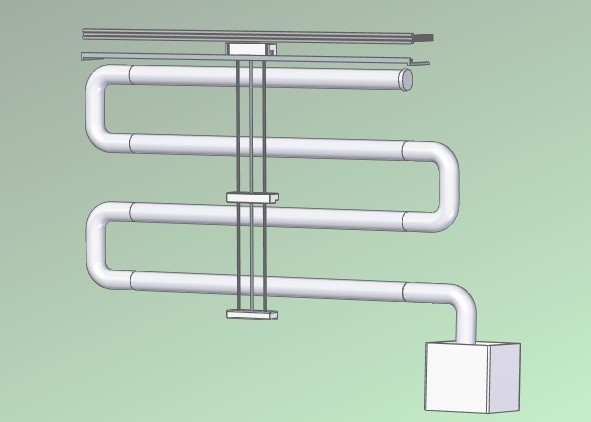
\includegraphics[width=0.35\textwidth]{img/ClaudioReal_simplificado.jpg}
        \caption{\textit{Representación de la estructura del cosechador automático y su entorno.}}
        \label{fig:ClaudioReal_simplificado}
\end{figure}
